\documentclass[10pt,a4paper]{article}

% Packages
\usepackage[utf8]{inputenc}
\usepackage{amssymb}
\usepackage{mathtools}
\usepackage{gensymb}
\usepackage{amsmath}
\usepackage{MnSymbol}

\title{\textbf{Mathematical proofs}}
\author{Michal Špano}
\date{March 2022}

\begin{document}

\maketitle

\section{The inner angle of an $n-sided$ convex regular polygon}

% Introduction
Suppose an $n-sided$ convex regular polygon. Its 4 consecutive vertices are shown in the figures, $N_1, N_2, N_3, ..., N_i$ respectively. 
Thus $\Delta_{N_1,N_2,S} \cong \Delta_{N_2,N_3,S}$, i.e. such $n-sided$ polygon consists of $n$ congruent isosceles triangles. 
That is, $|\measuredangle N_2 N_1 S| = |\measuredangle N_1 N_2 S| \implies |\measuredangle N_1 N_2 S| = |\measuredangle S N_2 N_3|$, denoted as $\beta, \beta'$ respectively. 

% Section I
An angle $\alpha = |\measuredangle N_1 S N_2| = \cfrac{360}{n}$, since such an angle multiplied by $n$ makes for a perfect circle of $360\degree$. Likewise $\alpha = 180\degree - 2 \beta$.

% Section I
Let $\Phi$ be an inner angle of the polygon, such that $\phi = 2 \beta$ (shown in the figure at the vertex $N_2$).

% Steps of computations
Express in terms of $\beta$: $\alpha = 180 - 2 \beta \iff \beta = \cfrac{-\alpha + 180}{2}$

Substitute $\alpha$ for $\alpha = \cfrac{360}{n}$: $\beta = \cfrac{-\cfrac{360}{n} + 180}{2} \iff \beta = \cfrac{180n - 360}{2n}$

Express in terms of $\Phi$: $\Phi = 2 \beta = 2 \Big( \cfrac{180n - 360}{2n} \Big) = \cfrac{180n - 360}{n}$ \\

The expression can be further simplified to the following form:

% End of the proof
$$\Phi = \cfrac{(n-2) \pi}{n}$$.

% Include a picture of a unit circle
\begin{figure}[htp]
    \centering
    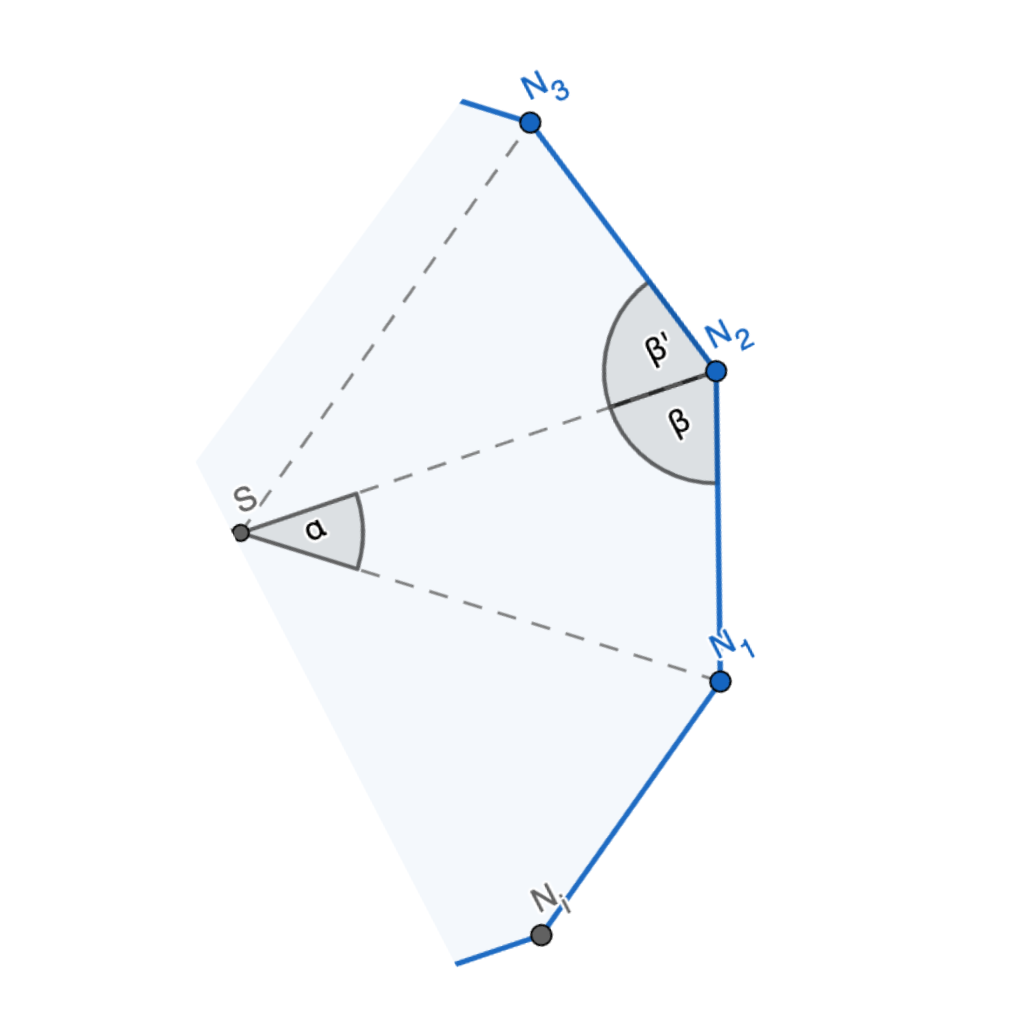
\includegraphics[width=4.cm]{polygon_export.png}
    \caption{$n-sided$ polygon with its 4 vertices in a plane}
\end{figure}

\newpage

\section{The number of diagonals of an $n-sided$ convex regular polygon}

Suppose a geometrical locus of $n$ points on the plane, 
% Steps of the proof
i.e. a set of points $A_1, A_2, ..., A_n$ 
such that $A_1, A_2, ..., A_n$ create an $n-sided$ convex regular polygon.
The number of different abscissas in the geometrical locus is ${n \choose 2}$ 
and denoted as $N_a$. It implies that no abscissa in the locus is given by more than two points, 
i.e. each point is unique. Likewise, $\overlinesegment{A_1A_2} \equiv \overlinesegment{A_2A_1}$ 
holds for any 2 points in the locus, thus such abscissas are counted as one. It can be inferred 
that the number of diagonals, denoted as $N_D$, is the same as \textit{the difference of the number of 
abscissas and the number of sides}: 

% End of the proof
$$N_D = N_s - n$$

\section{The similarity coefficient}

% Start of the proof
Suppose a scalene triangle $\Delta_{ABC}$. We assume that there exists a triangle $\Delta_{A'B'C'}$,
such that $\Delta_{ABC} \cong \Delta_{A'B'C'}$. It implies that there exists some constant $c$,
such that any abscissa created in the locus of points (from the original triangle) is equal to the
product of $c$ and the corresponding abscissa of the similar triangle. Symbolically: 

% General expression
$\exists! c \in \mathbb{Q}: |V_1 V_2| = c \times |V_1' V_2'| \land c \gneqq 1$, where $V_1, V_2$ 
are the vertices of the original triangle.

% Section 1 - perimeters
Then, it can be easily inferred, that for the \textbf{perimeters} of the triangles 
holds the following: Let $P = \overlinesegment{AB} + \overlinesegment{BC} + \overlinesegment{AC}$, similarly 
$P' = \overlinesegment{A'B'} + \overlinesegment{B'C'} + \overlinesegment{A'C'}$. Likewise
% Enumerating the similar sides with a constant
$
\overlinesegment{AB} = c \times \overlinesegment{A'B'} \land 
\overlinesegment{BC} = c \times \overlinesegment{B'C'} \land
\overlinesegment{AC} = c \times \overlinesegment{A'C'}
$. \\

% Steps of computation - perimeter
$P = c \times \overlinesegment{A'B'} + c \times \overlinesegment{B'C'} + c 
\times \overlinesegment{A'C'} \implies$
$P = c \times \Big( \overlinesegment{A'B'} + \overlinesegment{B'C'} + \overlinesegment{A'C'} \Big) = c \times P'$

$$P = c \times P'$$.

% Conclusion of section 1
It implies that the ratio of the lengths of the sides of the similar triangles, 
i.e. the ratio of their perimeters, is equal to the similarity coefficient:
$c = \cfrac{P}{P'}$. \\

% Section 2 - areas
Similar methodology is applied to the similarity coefficient of the areas of the triangles:

% Steps of computation - area
Let $
A = \dfrac{\overlinesegment{AB} \times \overlinesegment{H_{AB}}}{2} \land 
A' = \dfrac{\overlinesegment{A'B'} \times \overlinesegment{H'_{AB}}}{2}$,
where $H_{AB}$ and $H'_{AB}$ are the heights of the triangles. Thus,
$A = \dfrac{c \times \overlinesegment{A'B'} c \times \overlinesegment{H'_{AB}}}{2} = 
c^2 \times \Bigg( \dfrac{\overlinesegment{A'B'} \times \overlinesegment{H'_{AB}}}{2} \Bigg) = c^2 \times A'$

$$A = c^2 \times A'$$

% Conclusion of section 2
It implies, that the ratio of the areas equals to the similarity coefficient 
taken to the second power: $c^2 = \cfrac{A}{A'}$. \\

% Conclusion
To sum up, such a methodology is also applicable to derive the similarity coefficient 
of the volume of the tetrahedron. Moreover, it is also applicable to derive the similarity coefficient
of any planar polygon or solid figure (a scalene triangle per the given example is just an exemplary instance). 
Still, the following holds: $P = c \times P' \land A = c^2 \times A' \land V = c^3 \times V'$ 
based on the principles of \textbf{congruence}.

% End of the proof

\end{document}
